% This is file JFM2esam.tex
% first release v1.0, 20th October 1996
%       release v1.01, 29th October 1996
%       release v1.1, 25th June 1997
%       release v2.0, 27th July 2004
%       release v3.0, 16th July 2014
%   (based on JFMsampl.tex v1.3 for LaTeX2.09)
% Copyright (C) 1996, 1997, 2014 Cambridge University Press

\documentclass{jfm}
\usepackage{graphicx}
\usepackage{epstopdf, epsfig}

\newtheorem{lemma}{Lemma}
\newtheorem{corollary}{Corollary}

\shorttitle{Sedimentation of filament with inhomogeneous mass and stiffness}
\shortauthor{M. Lauber, G. D. Weymouth}

\title{Filemant sedimentation with inhomogeneous mass and stiffness distribution}

\author{Marin Lauber\aff{1}
  \corresp{\email{M.Lauber@tudelft.nl}},
  \and G. D. Weymouth\aff{1}}

\affiliation{\aff{1}Ship Hydromechanics, Department of Maritime Transport Technology, Faculty of Mechanical Engineering, Delft University of Technology,
Delft, Netherlands}

\begin{document}

\maketitle

\begin{abstract}
This file contains instructions for authors planning to submit a paper to the {\it Journal of Fluid Mechanics}. These instructions were generated in {\LaTeX} using the JFM style, so the {\LaTeX} source file can be used as a template for submissions. The present paragraph appears in the \verb}abstract} environment. All papers should feature a single-paragraph abstract of no more than 250 words, which provides a summary of the main aims and results. 
\end{abstract}

\begin{keywords}
Sedimentation, fluid-structure, simulation
\end{keywords}

\section{Introduction}

\citep{Tam2015FlexibilityWings}

\section{Method}

We perform two-dimensional (2D) numerical simulation of the filament sedimentation by solving the \emph{Navier-Stokes} equations for an inexpressible flow on a Cartesian mesh. The filament is immersed into the grid using the BDIM-$\sigma$ \citep{Lauber2022} that allows to accurately model thin, flexible immersed objects without a slip error on the filament's surface. We use a domain of size $mL\times nL$ with far-field boundary conditions (see~Sec.~\ref{sec:far-field}) to completely remove the domain's influence on the flow field.

Strong coupling with the structural equations describing the filament's motion is achieved through a Quasi-Newton approach \citep{Degroote2008AnInteraction} that uses the \citep{Lauber2023Immersed-BoundaryShells}

\subsection{Isogeometric filaments}

We model the filaments as initially straight beams with constant cross-section area but varying stiffness and density distributions. Under these assumptions, we can model the response of the filament to an external (fluid) force as a non-linear Euler-Bernoulli beam
\begin{equation}
    EIw'''' = F_{ext}
\end{equation}
A Non-uniform rational B-Splines (NURBS) curve of degree $p$ is defined as
\begin{equation}
    C(u) = \sum_{i=1}^{n} R_{i,p}(u)P_i
\end{equation}
where $R_{i,p}$ is the $i^{th}$ NURBS basis function of degree $p$ and is defined as
\begin{equation}\label{eq:nurbs_basis}
    R_{i,p}(u) = \frac{N_{i,p}(u)w_i}{\sum_{j=1}^{n}N_{j,p}(u)w_j}.
\end{equation}
Expression of the $p-1$ derivatives of the curve is easily obtained as
\begin{equation}
    C'(u) = \sum_{i=1}^{n} R'_{i,p}(u)P_i,
\end{equation}
where $R'_{i,p}(u)$ is the derivative of the NURBS basis function, obtained from application of the quotient rule to Eq.~\ref{eq:nurbs_basis}.\\

For a thorough introduction to isogeometric analysis, we refer the reader to \cite{Cottrell2006IsogeometricVibrations}. The advantage of isogeometric analysis over standard finite-element approaches is that, first, because of the nature of the NURBS basis function, very high continuity can be achieved between elements with ease ($C^{p-1}$). This results in continuous resolution of the frequency spectrum, which leads to better vibration frequency resolution compared to finite element analysis. Another advantage of IGA is that it drastically reduces the number of degrees of freedom of the structural system at equivalent accuracy.

\subsection{Moving reference frame and Biot-Savart boundary conditions}\label{sec:far-field}
Tracking the motion of the filament following its center of mass requires accelerating the frame of reference of the fluid domain using the filament's instantaneous acceleration. With the immersed-boundary approach used here, the local deformation and rotational acceleration of the filament are modeled with the immersed boundary, while the linear acceleration of its center of mass is used to determine the acceleration of the fluid domain. In addition, we use the \emph{Biot-Savart} potential flow boundary condition developed in \emph{Weymouth and Lauber (2024)} to reduce the required size of the domain while removing the influence of the wall onto the solution.\\
We start by describing, in words, how we coupled the moving reference frame and the \emph{Biot-Savart} boundary conditions to the implicit time integration of the coupled fluid-structure interaction system.\\
Integration of a single time step, from $t\to t+\Delta t$, starts by storing the flow fields (velocity $\vec u$ and pressure $p$) and the structural position ($\vec{s}$), velocity ($\dot{\vec{s}}$) and acceleration ($\ddot{\vec{s}}$). Next, the velocity of the fluid domain is set using the velocity of the filament's center of mass ($\vec{U}=\int_{0}^{L}\dot{\vec s}(\xi)d\xi/L$), serving as the potential flow boundary condition for the whole implicit step. We then proceed to solve the coupled fluid-structure system. A Jacobi method is used to predict the flow field and structural quantities at $t+\Delta t$. These new field quantities are used to compute structural displacement and fluid forces that are then compared to the one used at the start of the time step. If these are sufficiently similar (following a relative residual criterion), the system is deemed converged, and we proceed to the next time step. If these are not converged, as is often the case after the first iteration, acceleration of the coupling variable is performed (IQN-ILS or relaxation) and these new structural deformation and fluid forces are used to repeat the time step, using the saved flow field and structural quantities. The procedure is repeated until convergence is achieved. Within the Jacobi step, the momentum equation of the \emph{Navier-Stokes} equation is solved with the \emph{Biot-Savart} boundary conditions injected into them. As described in \emph{Weymouth and Lauber (2024)}, this requires solving a coupled pressure-boundary conditions system. A pseudo-algorithm is shown on Fig~\ref{fig:fsi-biot-MRF}

\begin{figure}
    \centering
    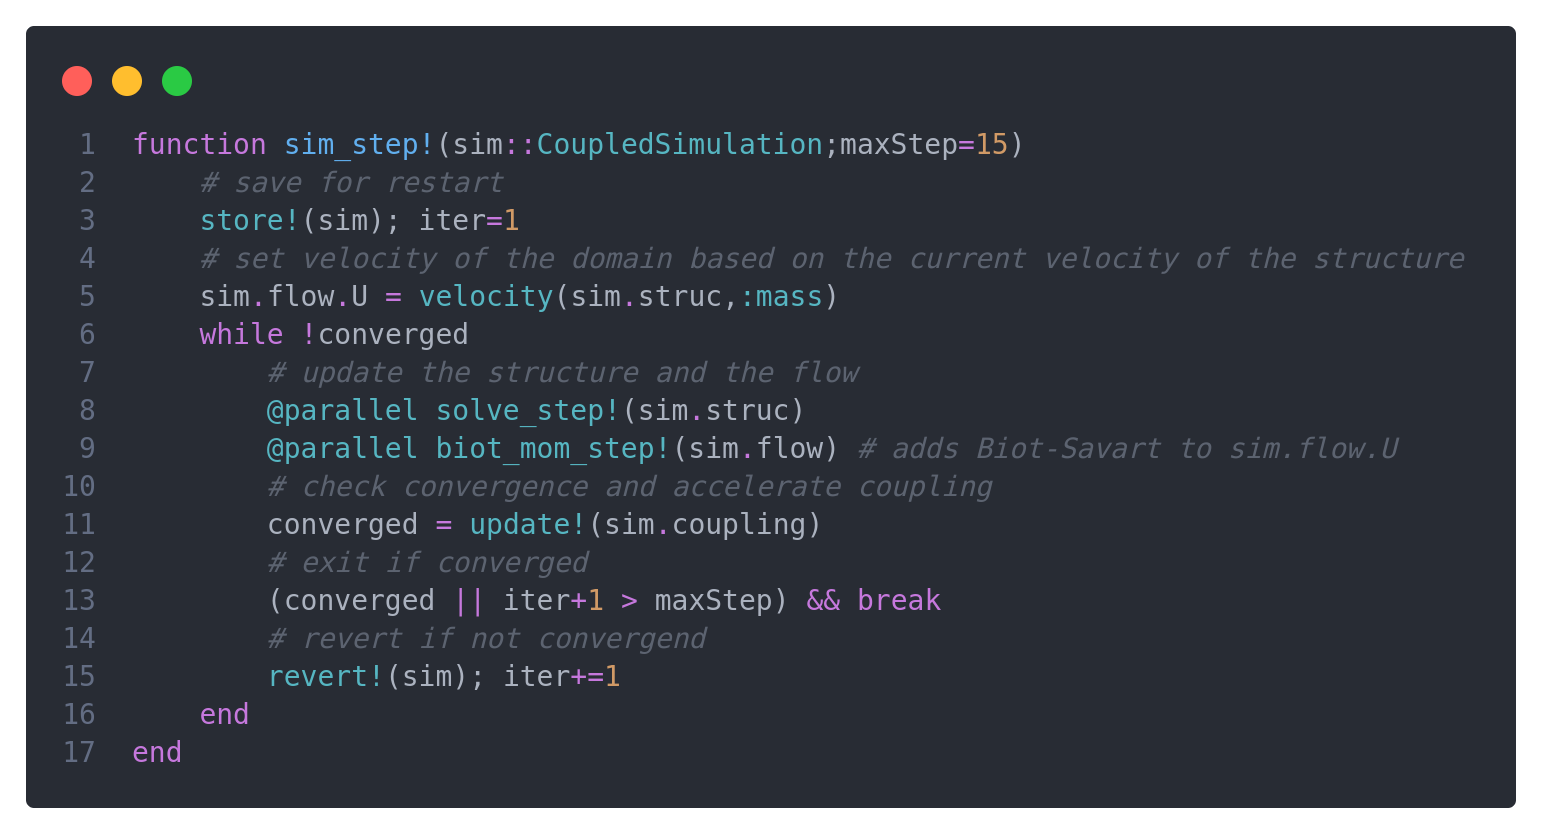
\includegraphics[width=\textwidth]{figures/code.png}
    \caption{Pseudo-code for the coupled fluid-structure interaction system with moving reference frame and \emph{Biot-Savart} boundary conditions.}
    \label{fig:fsi-biot-MRF}
\end{figure}

\section{Results}

\section{Conclusion}

\bibliographystyle{jfm}
% Note the spaces between the initials
\bibliography{references}

\end{document}
